\chapter{Analisi Semantica}\label{chap:semantical}
%
\vspace*{-2ex}
\begin{center}

\includegraphics[width=5.5cm]{ThinkingCat.png}
\end{center}
%\vspace*{-2ex}
%
Le analisi lessicale e sintattica dei Capitoli~\ref{chap:lexical}
e~\ref{chap:syntactical} garantiscono che il programma sorgente
soddisfi le regole di sintassi specificate, rispettivamente,
da un insieme di token e da una grammatica. L'analisi sintattica
ha inoltre costruito un albero di sintassi astratta che fornisce una visione
strutturata del file sorgente (Figura~\ref{fig:led_albero}).
Questo non significa che tutti i programmi che hanno superato con successo
l'analisi sintattica, \cioe senza generare alcun errore di sintassi,
siano automaticamente dei programmi \emph{corretti}, pronti ad essere tradotti
in codice oggetto ed eseguiti. Per esempio, basta prendere il programma
della Figura~\ref{fig:led} e modificare la linea \texttt{this.state := true}
in \texttt{this.state := 3} per ottenere un programma che supera senza alcun
problema sia l'analisi lessicale che quella sintattica, ma che non \`e
\emph{corretto}, poich\'e esso tenta di assegnare un valore intero
($3$) a un campo che pu\`o contenere solo valori di tipo
booleano (\texttt{state}). Accorgersi di tali errori va ben al di l\`a delle
possibilit\`a delle grammatiche libere dal contesto. Serve uno strumento
alternativo, ovvero quello della discesa ricorsiva sull'albero di sintassi
astratta del codice sorgente, alla ricerca di errori \emph{semantici}
nel codice. Questa \emph{analisi semantica} \e l'oggetto di questo capitolo.

Pi\`u in dettaglio, i compiti di un'analisi semantica sono quelli di
%
\begin{enumerate}
\item costruire una rappresentazione (una struttura dati) che descrive
      i tipi usati dal programma (tipi primitivi ma anche array e classi);
\item identificare usi di espressioni incompatibili con i loro tipi statici
      (\emph{errori di tipo});
\item identificare occorrenze di variabili usate ma non dichiarate;
%\item garantire che i comandi \texttt{break} e \texttt{continue} occorrano
%      solo nello scope di un'istruzione iterativa;
\item garantire che un metodo non \texttt{void} termini sempre con
      un comando \texttt{return} \textit{exp},
      indipendentemente dal percorso di
      esecuzione che viene seguito al suo interno, e che un metodo
      \texttt{void} non contenga comandi di tipo \texttt{return} \textit{exp};
\item garantire che non ci siano parti di codice che non possono mai
      essere eseguite e che sono quindi irraggiungibili e \emph{inutili}
      (identificazione \emph{del codice morto});
\item identificare e annotare il tipo statico delle espressioni che occorrono
      in un programma (\emph{inferenza dei tipi});
\item identificare, per ogni accesso a un campo, la classe in cui il campo
      \`e definito;
\item identificare per ogni istruzione \texttt{new} \textit{Classe},
      sulla base del tipo statico dei parametri attuali,
      il costruttore di \textit{Classe}
      che deve essere chiamato in tale punto a tempo di esecuzione;
\item identificare per ogni invocazione di metodo, sulla base del tipo statico
      dei parametri attuali, la dichiarazione del metodo
      che deve essere chiamato (o una cui ridefinizione deve essere chiamata)
      in tal punto a tempo di esecuzione.
\end{enumerate}
%
Potremmo quindi dire che l'analisi semantica si occupa di
costruire una rappresentazione dei tipi usati dal programma (punto 1)
che viene poi usata per garantire condizioni
di correttezza elementari, senza le quali non ha neppure senso compilare
il programma in codice oggetto (\emph{verifica del codice},
punti 2--5) e per raccogliere informazione
sul programma che si sta compilando, al fine di facilitare la successiva
fase di generazione del codice oggetto (\emph{annotazione del codice},
punti 6--9). Va detto che tale
divisione \`e concettualmente utile ma non netta, dal momento che, per
esempio, l'identificazione del costruttore chiamato da un'istruzione
\texttt{new} (punto 8) \`e s\`{\i} un'annotazione utile a
generare il codice oggetto
che effettua la chiamata a tale costruttore, ma \`e anche una verifica che
tale costruttore esista realmente. L'insieme esatto
dei compiti affidati all'analisi semantica varia comunque molto da
linguaggio a linguaggio.
Altre verifiche effettuate da Java \emph{ma non da Kitten} sono per esempio:
%
\begin{enumerate}
\item[10.] garantire che i comandi \texttt{break} e \texttt{continue}
           occorrano solo dentro un costrutto iterativo o, per il solo
           \texttt{break}, dentro un comando \texttt{switch};
\item[11.] garantire che l'uso di una variabile locale trovi la variabile
           inizializzata, indipendentemente dal percorso di esecuzione
           che ha portato al punto di utilizzo della variabile\footnote
           {In Kitten una variabile va inizializzata al momento
           della sua dichiarazione, per cui questo controllo \e inutile.}.
\end{enumerate}
%
\section{I tipi Kitten}\label{sec:semantical_types}
%
Il concetto di \emph{tipo} (Sezione~\ref{sec:types}) \`e al centro
dell'analisi semantica (punti 1,2,4,6,8,9 della precedente
enumerazione). Va subito notato che per \emph{tipo}
non intendiamo qui la sintassi
astratta di una \emph{espressione} di tipo, come nella
Sezione~\ref{subsec:types_abstract}. In quel contesto avevamo bisogno di
un modo per rappresentare la \emph{struttura sintattica} di una parte di codice
che rappresentava un tipo Kitten. Si tratta invece adesso di rappresentare
la \emph{struttura semantica} dei tipi delle espressioni Kitten,
\cioe una struttura dati con associate alcune operazioni
che permettono, per esempio, di determinare se un tipo \`e un sottotipo
di un altro o qual \`e il minimo supertipo
comune fra due o \piu tipi, se esso esiste (Sezione~\ref{sec:types}), o quali
sono i campi o i costruttori o metodi di un tipo classe.
Per apprezzare la differenza, basta osservare che
due occorrenze dell'espressione \texttt{int} in due punti diversi
di un file sorgente danno origine a due oggetti \texttt{IntTypeExpression}
diversi, ma il loro tipo semantico \`e lo stesso identico oggetto.

La distribuzione Kitten contiene il package \texttt{types}, al cui interno
trovano posto delle classi che rappresentano i tipi \emph{semantici}
del linguaggio Kitten.
%
\begin{figure}
\begin{center}
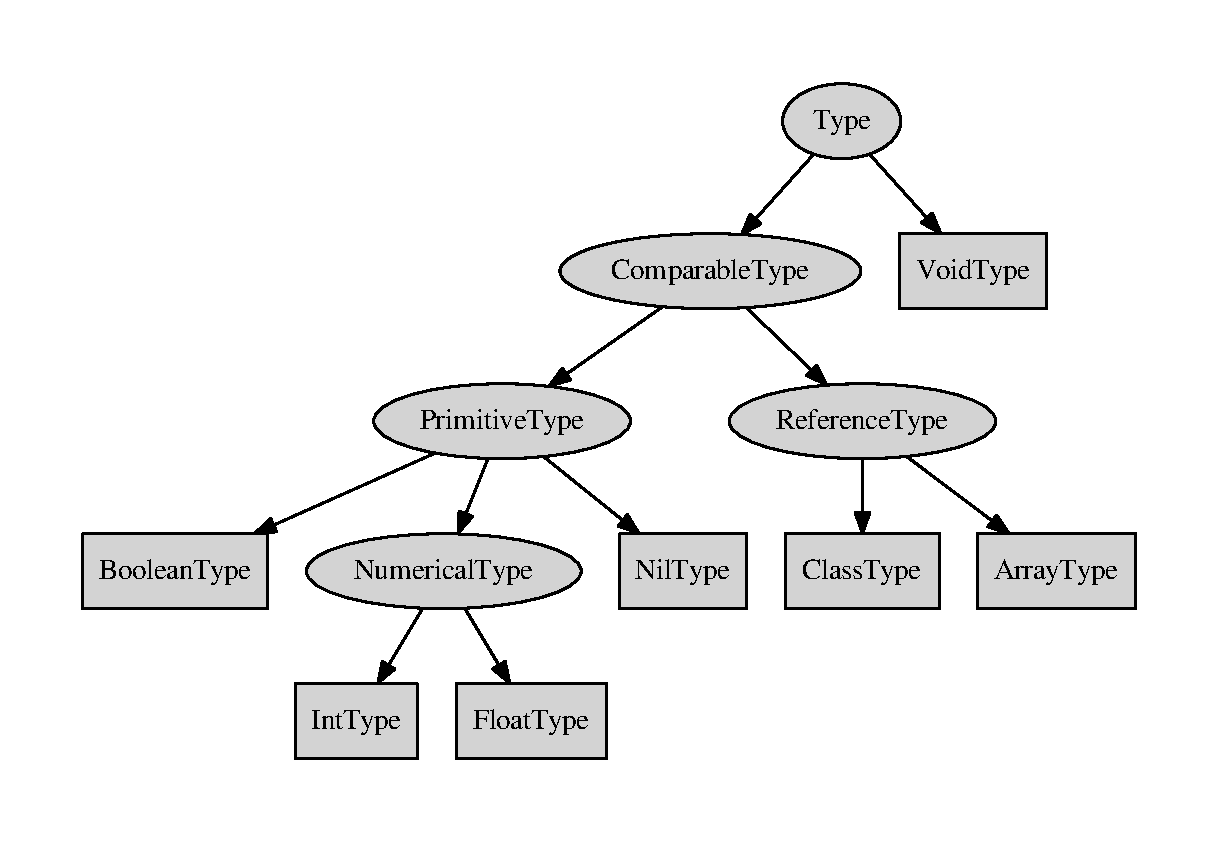
\epsfig{file = semantical_types.pdf, width = 12cm}
\end{center}
\caption{Le classi del package \texttt{types} che rappresentano i tipi semantici di Kitten.}\label{fig:semantical_types}
\end{figure}
%
La Figura~\ref{fig:semantical_types} presenta la gerarchia di tali classi.
I tipi sono in primo luogo divisi fra \emph{confrontabili} e \texttt{void}.
I tipi confrontabili sono quelli per i cui valori \`e definito almeno
l'operatore di confronto \texttt{=}. Essi sono a loro volta divisi fra
tipi \emph{primitivi} e \emph{riferimento} (Sezione~\ref{sec:types}). I tipi
\emph{numerici} sono quei tipi primitivi che rappresentano numeri e per
cui sono definite le usuali operazioni di confronto, come il \texttt{<},
oltre a \texttt{=}.
Si noti che non esiste un tipo specifico per le stringhe, che sono invece
considerate come un caso di \texttt{ClassType}.

La Figura~\ref{fig:types.Type} mostra l'implementazione della superclasse
\texttt{types/Type.java}. Essa definisce in primo luogo delle costanti
per dei tipi di uso comune. Le sue sottoclassi dovranno istanziare
il metodo \texttt{canBeAssignedTo()} che determina
se un tipo pu\`o essere assegnato a un
altro, seguendo le regole che nella Sezione~\ref{sec:types}
hanno portato alla definizione della relazione $\le$ sui tipi. Il metodo
\texttt{canBeAssignedToSpecial()} \e per default un sinonimo di
\texttt{canBeAssignedTo()}, ma viene ridefinito in
\texttt{types/PrimitiveType.java} e \texttt{types/Void.java} come segue:
%
\begin{verbatim}
  public boolean canBeAssignedToSpecial(Type other) {
    return this == other;
  }
\end{verbatim}
%
in modo che i tipi primitivi e \texttt{void} siano
\emph{sottotipo speciale} solo di se stessi. Questo metodo \`e
utile all'interno della classe \texttt{ArrayType}, che vedremo fra un attimo,
per implementare la relazione di sottotipaggio $\le$ che come sappiamo
non \`e monotona sugli array di tipi primitivi (Sezione~\ref{sec:types}).
Esso \e usato anche per determinare se il tipo di ritorno di una ridefinizione
di un metodo \`e compatibile con quello del metodo ridefinito.
Il metodo \texttt{leastCommonSupertype()} determina il minimo supertipo comune
fra due tipi. Tale supertipo potrebbe non esistere: fra
\texttt{int} e \texttt{boolean} non c'\e alcun supertipo comune.
La definizione fornita dentro
\texttt{types/Type.java} funziona per tutti i tipi primitivi, ma come
vedremo deve essere ridefinita per i tipi riferimento.
Si noti che il costruttore di \texttt{types/Type.java} \`e \texttt{protected}.
Anche i costruttori delle altre classi che implementano i tipi semantici sono
\texttt{protected} o \texttt{private}. Quindi
l'unico modo per ottenere degli oggetti della
gerarchia in Figura~\ref{fig:semantical_types} sar\`a tramite le costanti
definite in Figura~\ref{fig:types.Type} o tramite
dei costruttori con memoria che
definiremo dentro le classi per i tipi riferimento. Questo implica
che \emph{esiste al pi\`u un oggetto per un dato tipo semantico}
e l'uguaglianza fra tipi pu\`o essere controllata con
semplici confronti Java \texttt{==}. Il metodo \texttt{getObjectType()}
ritorna il tipo della superclasse \texttt{Object} di tutte le classi ed array.

\begin{figure}[t]
{\small
\begin{verbatim}
public abstract class Type {
  // delle costanti di uso frequente
  public final static BooleanType BOOLEAN = new BooleanType();
  public final static FloatType FLOAT = new FloatType();
  public final static IntType INT = new IntType();
  public final static NilType NIL = new NilType();
  public final static VoidType VOID = new VoidType();

  protected Type() {}
  public abstract boolean canBeAssignedTo(Type other);
  public boolean canBeAssignedToSpecial(Type other) {
    return canBeAssignedTo(other); // i tipi primitivi lo ridefiniscono
  }
  public Type leastCommonSupertype(Type other) {
    // questo e' ok per i tipi primitivi. Classi e array lo ridefiniscono
    if (this.canBeAssignedTo(other)) return other;
    else if (other.canBeAssignedTo(this)) return this;
    else return null; // non esiste
  }
  public static final ClassType getObjectType() { ... ritorna il tipo per Object }
}
\end{verbatim}
}
\caption{La superclasse astratta dei tipi semantici di Kitten}
  \label{fig:types.Type}
\end{figure}

Si consideri la classe \texttt{types/IntType.java}
in Figura~\ref{fig:types.IntVoidType}.
Come si vede, ammettiamo che il tipo \texttt{int} sia assegnato a
\texttt{int} stesso ma anche a \texttt{float}, poich\'e
$\mathtt{int}\le\mathtt{float}$ (Sezione~\ref{sec:types}).
La classe \texttt{types/VoidType.java} \`e simile, ma non ammettiamo
l'assegnamento verso nessun tipo, neppure \texttt{void}.
L'assegnamento speciale \`e invece possibile ma solo verso \texttt{void}
stesso, come abbiamo gi\`a detto.
%
\begin{figure}
{\small
\begin{verbatim}
           public class IntType extends NumericalType {
             protected IntType() {}
             public boolean canBeAssignedTo(Type other) {
               return other == Type.INT || other == Type.FLOAT;
             }
           }

           public class VoidType extends Type {
             protected VoiType() {}
             public boolean canBeAssignedTo(Type other) { return false; }
             public boolean canBeAssignedToSpecial(Type other) {
                 return this == other;
             }
           }
\end{verbatim}}
\caption{Le classi \texttt{types/IntType.java} e
         \texttt{types/VoidType.java} che implementano rispettivamente i tipi
         \texttt{int} e \texttt{void}.}
  \label{fig:types.IntVoidType}
\end{figure}

\greycomment{
La scelta di imporre l'uguaglianza nella relazione di sottotipo speciale
per i tipi primitivi ha l'effetto che, nel controllo di compatibilit\`a
del tipo di ritorno della ridefinizione di un metodo, un tipo primitivo pu\`o
essere solo sottotipo di se stesso. Si osservi che se \texttt{float m()}
potesse essere ridefinito, in una sottoclasse, in \texttt{int m()}
allora una chiamata virtuale del tipo \texttt{float f = o.m()} richiederebbe,
o meno, una conversione di tipo da \texttt{int} a \texttt{float} sulla base
della classe, a tempo di esecuzione, dell'oggetto contenuto in \texttt{o}, il
che complica la generazione del codice. Quindi impediamo al programmatore di
fare una simile ridefinizione del tipo di ritorno del metodo \texttt{m()}.
Questo stesso vincolo \e imposto nel linguaggio Java.}

\begin{figure}[t]
{\small
\begin{verbatim}
public class ArrayType extends ReferenceType {
  private Type elementsType;
  private ArrayType(Type elementsType) { this.elementsType = elementsType; }
  public static ArrayType mk(Type elementsType) {
    ... usa una memoria per non ricreare tipi array gia' creati in passato
  }
  public boolean canBeAssignedTo(Type other) {
    if (other instanceof ArrayType)
      return elementsType.canBeAssignedToSpecial(((ArrayType)other).elementsType);
    else return other == getObjectType();
  }
  public Type leastCommonSupertype(Type other) {
    // l'lcs fra un array e una classe e' Object
    if (other instanceof ClassType) return getObjectType();
    else if (other instanceof ArrayType)
      if (elementsType instanceof PrimitiveType)
        // fra un array di tipi primitivi e se stesso l'lcs e' l'array.
        if (this == other) return this;
        // fra due array di tipi primitivi diversi, l'lcs e' Object
        else return getObjectType();
      else {
        Type lcs = elementsType.leastCommonSupertype(((ArrayType)other).elementsType);
        if (lcs == null) return getObjectType();
        else return mk(lcs);
      }
    else if (other == Type.NIL) return this; // fra un array e nil e' l'array
    else return null; // non esiste alcun lcs
  }
}
\end{verbatim}
}
\caption{La classe \texttt{types/ArrayType.java} che rappresenta i tipi array.}\label{fig:types.ArrayType}
\end{figure}

La classe \texttt{types/ArrayType.java} in Figura~\ref{fig:types.ArrayType}
implementa i tipi array. L'invariante che
non esistano istanze diverse dello stesso tipo \`e mantenuta rendendone
\texttt{private} il costruttore e permettendo la
creazione di tipi array solo tramite il metodo statico \texttt{mk()}, che
usa una memoria per evitare di creare duplicati.
L'assegnamento di un tipo array \texttt{this}
a un altro tipo \texttt{other} \`e considerata
legale solo se \texttt{other} \`e \texttt{Object} oppure se anche
\texttt{other} \`e un tipo array e gli elementi di \texttt{this}
possono a loro volta essere assegnati a quelli di \texttt{other}.
Ma si noti l'uso di \texttt{canBeAssignedToSpecial()} per questa chiamata
ricorsiva! Questo al fine di imporre il vincolo
della Sezione~\ref{sec:types} che richiede che se gli elementi
di \texttt{this} sono un tipo primitivo allora quelli di \texttt{other} devono
essere \emph{lo stesso} tipo primitivo.
%
\greycomment{Questo vincolo, apparentemente strano, \`e giustificato dal fatto
che se \texttt{arr} \`e un array di interi allora
il comando \texttt{int[] copy := arr}
rende \texttt{arr} e \texttt{copy} \emph{alias}, \cioe riferimenti diversi
allo stesso oggetto array. Mentre il comando \texttt{float[] copy := arr}
ci impone di convertire ciascun elemento di \texttt{arr} da \texttt{int}
a \texttt{float}. Dal momento che dobbiamo lasciare immutato l'array
\texttt{arr}, la conversione \`e possibile solo a costo di creare
un \emph{nuovo} array di \texttt{float} che contiene i valori convertiti.
Tale array verrebbe poi assegnato a \texttt{copy}. Ma questo significa
che \texttt{arr} e \texttt{copy} non sarebbero \piu alias! Detto
altrimenti, la scelta del tipo degli elementi di \texttt{copy} determinerebbe
la condivisione (o meno) fra \texttt{arr} e \texttt{copy}. Tale comportamento,
nettamente inaspettato dal programmatore, \`e da considerarsi
semanticamente pericoloso ed
\`e quindi conveniente vietare tali assegnamenti. Va notato inoltre che il
costo computazionale dell'assegnamento diventerebbe lineare nella lunghezza
dell'array piuttosto che costante, come normalmente si richiede.}

Il metodo \texttt{leastCommonSupertype()} di
\texttt{ArrayType} deve determinare il minimo supertipo comune
(\emph{lcs}) fra il tipo array \texttt{this} e un altro tipo \texttt{other}.
Le regole che portano alla definizione di \emph{lcs} sono le seguenti:
%
\begin{itemize}
\item se \texttt{other} \`e una classe allora \emph{lcs} \`e \texttt{Object}.
      Si noti infatti che tutti gli array e tutte le classi sono
      sottotipi di \texttt{Object} (Sezione~\ref{sec:types});
\item se anche \texttt{other} \`e un tipo array allora:
      \begin{itemize}
      \item se entrambi sono array dello stesso tipo primitivo
            allora \emph{lcs} \`e uguale
            a \texttt{this} (o equivalentemente a \texttt{other});
      \item se entrambi sono array di tipi primitivi diversi
            allora \emph{lcs} \`e \texttt{Object}; si noti che sarebbe
            errato definire in questo caso \emph{lcs} come
            \texttt{array of Object}, poich\'e i tipi primitivi non sono
            sottotipi di \texttt{Object};
      \item se entrambi sono array di tipi non primitivi
            allora \emph{lcs} \`e il tipo array del minimo supertipo comune
            fra i tipi degli elementi di \texttt{this} e \texttt{other};
      \end{itemize}
\item se \texttt{other} \`e il tipo \texttt{NilType}, allora
      \emph{lcs} \`e \texttt{this} poich\'e \texttt{NilType} \`e un
      sottotipo di qualsiasi tipo array (Sezione~\ref{sec:types});
\item altrimenti \emph{lcs} non esiste.
\end{itemize}

\begin{figure}[t]
{\scriptsize
\begin{verbatim}
public class ClassType extends ReferenceType {
  private Symbol name;                    // il nome di questa classe
  private ClassType superclass;           // la sua superclasse (se esiste)
  private ClassTypeList subclasses;       // le sue sottoclassi (se esistono)
  private Parser parser;                  // il parser usato per questa classe
  private ClassDefinition abstractSyntax; // la sintassi astratta della classe

  private ClassType(Symbol name) {
    ... salva this nella memoria usata da mk()
    this.name = name; parser = new Parser(new Lexer(name));
    (abstractSyntax = (ClassDefinition)parser.parse().value).addMembers(this);
    if (name != Symbol.OBJECT) {
      superclass = mk(abstractSyntax.getSuperclassName());
      superclass.subclasses = new ClassTypeList(this,superclass.subclasses);
    }
  }
  public static ClassType mk(Symbol name) {
    ... restituisci l'eventuale classe di nome name contenuta nella memoria
    ... altrimenti restituisci new ClassType(name)
  }
  public FieldSignature fieldLookup(Symbol name) { ... }
  public ConstructorSignature constructorLookup(TypeList formals) { ... }
  public HashSet constructorsLookup(TypeList formals) { ... }
  public MethodSignature methodLookup(Symbol name, TypeList formals) { ... }
  public HashSet methodsLookup(Symbol name, TypeList formals) { ... }
  public boolean canBeAssignedTo(Type other) {
    return other instanceof ClassType && this.subclass((ClassType)other);
  }
  public boolean subclass(ClassType other) {
    return this == other || (superclass != null && superclass.subclass(other));
  }
  public Type leastCommonSupertype(Type other) {
    if (other instanceof ArrayType) return getObjectType();
    else if (other instanceof ClassType)
      for (ClassType cursor = this; cursor != null; cursor = cursor.superclass)
        if (other.canBeAssignedTo(cursor)) return cursor;
    else if (other == Type.NIL) return this; else return null;
  }
}
\end{verbatim}
}
\caption{La classe \texttt{types/ClassType.java} che implementa il tipo classe di Kitten.}
  \label{fig:types.ClassType}
\end{figure}

Vediamo infine il tipo \texttt{ClassType}, che rappresenta i tipi
classe come \texttt{Object},
\texttt{String} o \texttt{Led} in Figura~\ref{fig:led}. La
Figura~\ref{fig:types.ClassType} ne riporta il codice. Il costruttore
\`e lasciato \texttt{private} e la costruzione di tipi classe \`e
possibile solo tramite il metodo statico \texttt{mk()} che ne garantisce
l'unicit\`a. Il costruttore si occupa di creare un analizzatore lessicale per
il file sorgente della classe, interfacciarlo con un analizzatore sintattico
ed effettuare il parsing sintattico della classe. La sintassi astratta \cosi
costruita \e memorizzata nel tipo classe. La costruzione prosegue con la
superclasse, di cui il nuovo oggetto diventa una sottoclasse.
Se non esistesse nessun file col nome della classe seguito
da \texttt{.kit} o se tale file contenesse degli errori di sintassi,
il metodo \texttt{parse()} del parser fallirebbe senza restituire alcuna
sintassi astratta. Tale eccezione sarebbe allora
intercettata da un gestore di eccezioni (non mostrato in
Figura~\ref{fig:types.ClassType}) che fornisce alla classe
una sintassi astratta minimale (superclasse \texttt{Object}, nessun
campo, n\'e costruttori, n\'e metodi). In questo modo si evita di
bloccare la compilazione di un programma soltanto perch\'e una della sue classi
contiene un errore: si va avanti con la compilazione
finch\'e si pu\`o, segnalando quanti \piu errori possibile al programmatore.

Un tipo classe ha informazione sulla \emph{segnatura}
della classe, \cioe sui suoi campi, costruttori e metodi.
Questa informazione \e estratta dalla sua sintassi astratta al momento
della costruzione di un tipo classe tramite il metodo
\texttt{addMembers()} a discesa ricorsiva
(Figura~\ref{fig:types.ClassType}). Si noti che se
i campi, costruttori o metodi fanno riferimento alla stessa classe che
stiamo creando non entriamo in loop poich\'e abbiamo avuto cura di
registrare il tipo classe che stiamo creando nella memoria di
\texttt{mk()} prima di chiamare \texttt{addMembers()}.

La segnatura della classe pu\`o essere
consultata in seguito tramite dei metodi di ricerca (\emph{lookup}).
La differenza fra i metodi
\texttt{constructorLookup()} e \texttt{constructorsLookup()} \`e che il
primo cerca il costruttore con parametri formali esattamente identici a quelli
indicati, mentre il secondo fornisce l'insieme $S$ di
\emph{tutti} i costruttori con parametri
formali aventi tipi compatibili con quelli indicati.
\`E garantito il vincolo che
nessun costruttore in $S$ ha un altro costruttore in $S$ con parametri
formali \piu specifici dei suoi. Per esempio, nella segnatura della classe:
%
\begin{verbatim}
  class Ambiguous {
    constructor(int i, float d) {}
    constructor(float d, int i) {}
    /* constructor(int i1, int i2) {} */
  }
\end{verbatim}
%
il risultato di \texttt{constructorsLookup()} con per parametro una lista di
due \texttt{IntType} \`e l'insieme dei
due costruttori della classe non commentati.
Entrambi sono infatti compatibili con
due parametri di tipo \texttt{int}. Se si eliminasse il commento intorno
al terzo costruttore, la stessa chiamata a \texttt{constructorsLookup()}
restituirebbe un insieme formato dal solo
terzo costruttore, che \`e \piu specifico degli altri due.
Si pu\`o adesso comprendere a cosa ci servir\`a il metodo
\texttt{constructorsLookup()}:
di fronte a una invocazione del costruttore di \texttt{Ambiguous},
del tipo \texttt{new Ambiguous(3,4)}, il compilatore Kitten
determina, tramite \texttt{constructorsLookup()}, l'insieme
dei possibili costruttori candidati a essere chiamati in tale punto di
programma. Se ce ne fosse \piu d'uno, la chiamata verrebbe considerata
\emph{ambigua}. Se non ce ne fosse nessuno, la
chiamata verrebbe considerata \emph{indefinita}.
In entrambi i casi essa verrebbe rifiutata in fase di analisi semantica
(lo vedremo quando commenteremo la Figura~\ref{fig:analysis_expressions2}).
Lo stesso discorso si pu\`o fare per
\texttt{methodLookup()} e \texttt{methodsLookup()}, con l'unica differenza che,
dal momento che Kitten implementa l'ereditariet\`a per campi e metodi,
la loro ricerca inizia in una data segnatura e,
se tale segnatura non definisce esplicitamente il campo o il metodo, la ricerca
prosegue ricorsivamente verso l'alto risalendo la catena delle estensioni,
verso \texttt{Object}.

Il metodo \texttt{canBeAssignedTo()} permette l'assegnamento verso la
stessa classe o una sua superclasse.
Il test di sottoclasse \`e realizzato dal metodo \texttt{subclass()}
che scorre verso l'alto a partire da \texttt{this}
la catena di estensione delle classi alla ricerca
dell'ipotetica superclasse.
Il metodo \texttt{leastCommonSupertype()} determina il minimo supertipo
comune \emph{lcs}
fra il tipo classe \texttt{this} e un altro tipo \texttt{other}
secondo le regole seguenti:
%
\begin{itemize}
\item se \texttt{other} \`e un tipo array, allora \emph{lcs} \`e
      \texttt{Object}, poich\'e tutte le classi e gli array sono
      sottotipi di \texttt{Object} (Sezione~\ref{sec:types});
\item se anche \texttt{other} \`e un tipo classe allora \emph{lcs}
      \`e la pi\`u specifica superclasse di \texttt{this} che \`e anche
      superclasse di \texttt{other}. Si noti che abbiamo la garanzia che
      tale \emph{lcs} esista poich\'e questa ricerca si ferma, nel
      peggiore dei casi, su \texttt{Object};
\item se \texttt{other} \`e il tipo \texttt{NilType}, allora
      \emph{lcs} \`e \texttt{this}, poich\'e \texttt{NilType} \`e
      sempre un sottotipo dei tipi classe (Sezione~\ref{sec:types});
\item altrimenti \emph{lcs} non esiste.
\end{itemize}
%
\begin{figure}[t]
\begin{center}
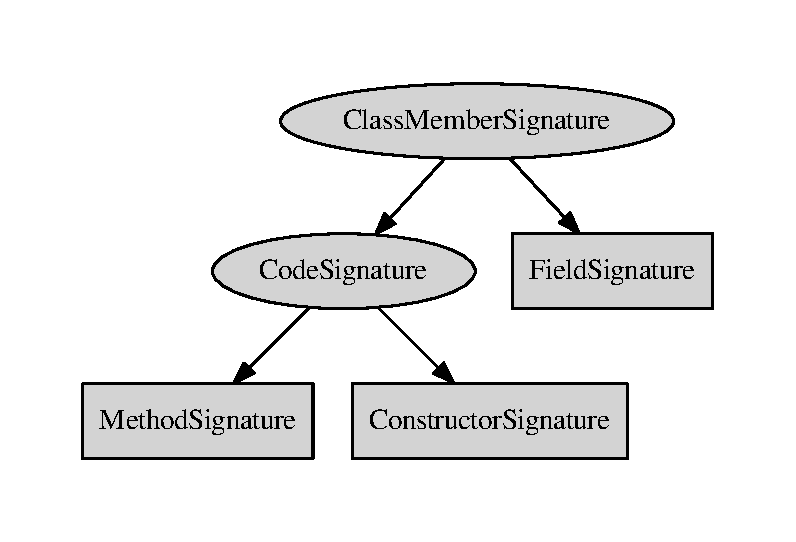
\epsfig{file = signatures_hierarchy.pdf, width = 8cm}
\end{center}
\caption{Le classi del package \texttt{types} che rappresentano le segnature dei membri di una classe.}\label{fig:signatures}
\end{figure}
%
\begin{figure}[t]
{\small
\begin{verbatim}
  public class FieldSignature extends ClassMemberSignature {
    private Type type;   // il tipo del campo
    private Symbol name; // il nome del campo
    public FieldSignature(ClassType clazz, Type type, Symbol name) {
      super(clazz); this.type = type; this.name = name;
    }
  }

  public abstract class CodeSignature extends ClassMemberSignature {
    private TypeList parameters; // i tipi dei parametri
    protected CodeSignature(ClassType clazz, TypeList parameters) {
      super(clazz); this.parameters = parameters;
    }
  }

  public class ConstructorSignature extends CodeSignature {
    public ConstructorSignature(ClassType clazz, TypeList parameters) {
      super(clazz,parameters);
    }
  }

  public class MethodSignature extends CodeSignature {
    private Symbol name;     // il nome del metodo
    private Type returnType; // il suo tipo di ritorno
    public MethodSignature
     (ClassType clazz, Type returnType, TypeList parameters, Symbol name) {
     super(clazz,parameters); this.name = name; this.returnType = returnType;
    }
  }
\end{verbatim}
}
\caption{Le classi che implementano le segnature dei membri di una classe Kitten.}
  \label{fig:members_signatures}
\end{figure}

La Figura~\ref{fig:types.ClassType} mostra che il tipo di ritorno dei metodi
di ricerca in una classe \e un oggetto (o un insieme di oggetti) di tipo
\texttt{FieldSignature}, \texttt{ConstructorSignature} o
\texttt{MethodSignature}. Tali classi implementano le \emph{segnature} di
campi, costruttori e metodi, rispettivamente, \cioe una specifica delle
loro propriet\`a di tipo. Per esempio, la segnatura di un campo di una classe
specifica il nome del campo, il suo tipo semantico di dichiarazione e
il tipo semantico della classe in cui il campo \`e definito.
%La segnatura di una classe \`e l'insieme delle
%segnature dei campi, costruttori e metodi che essa definisce,
%\piu un riferimento alla segnatura della sua superclasse, se esiste.

La Figura~\ref{fig:signatures} mostra la gerarchia delle
classi del package \texttt{types}
che rappresentano le segnature di campi, costruttori e metodi Kitten.
La Figura~\ref{fig:members_signatures} ne mostra l'implementazione. La
superclasse comune \texttt{types/ClassMemberSignature.java} (non mostrata in
Figura~\ref{fig:members_signatures}) descrive
la segnatura di un membro di una classe. Essa contiene semplicemente un
riferimento al tipo classe a cui il membro appartiene, inizializzato
dal costruttore. La classe \texttt{FieldSignature}
ha in \piu il tipo e nome del campo descritto. La classe
\texttt{CodeSignature} ha invece una lista di tipi, corrispondenti
ai tipi dei parametri formali del costruttore o metodo
che essa rappresenta. La classe \texttt{ConstructorSignature}
\e una estensione di \texttt{CodeSignature} che non aggiunge alcun
campo, mentre \texttt{MethodSignature} specifica anche il nome e il tipo di
ritorno del metodo.
%
\section{L'analisi semantica delle espressioni di tipo Kitten}\label{sec:analysis_types}
%
Effettuare l'analisi semantica dei tipi Kitten significa costruire il tipo
semantico $\st{t}$ rappresentato da ogni espressione sintattica di tipo $t$
che occorre nel programma e annotare tale tipo dentro $t$ stessa. La
costruzione di $\st{t}$ \e formalizzata nella Figura~\ref{fig:analysis_types}.
%
\begin{figure}
\begin{align*}
  \st{\_}:\mathtt{absyn.TypeExpression}&\mapsto\mathtt{types.Type}\\
  \mbox{}\\
  \st{\mathtt{IntTypeExpression()}}&=\mathtt{Type.INT}\\
  \st{\mathtt{FloatTypeExpression()}}&=\mathtt{Type.FLOAT}\\
  \st{\mathtt{BooleanTypeExpression()}}&=\mathtt{Type.BOOLEAN}\\
  \st{\mathtt{VoidTypeExpression()}}&=\mathtt{Type.VOID}\\
  \st{\mathtt{ArrayTypeExpression(\mathit{elementsType})}}
    &=\mathtt{ArrayType.mk(\st{\mathit{elementsType}})}\\
  \st{\mathtt{ClassTypeExpression(\mathit{name})}}
    &=\mathtt{ClassType.mk(\mathit{name})}
\end{align*}
\caption{La funzione di analisi semantica $\st{\_}$ per le espressioni di tipo Kitten.}\label{fig:analysis_types}
\end{figure}
%
Le espressioni di tipo che rappresentano i tipi primitivi
vengono mappate in costanti della classe
\texttt{types.Type}. Quelle che rappresentano gli array
vengono mappate in tipi semantici di tipo \texttt{types.ArrayType} per
il tipo semantico dei propri elementi.
Le espressioni di tipo che rappresentano un tipo classe vengono mappate
nell'oggetto di tipo \texttt{types.ClassType} per il nome della classe.
%Occorre inoltre segnalare un errore se per
%qualche tipo classe $\kappa$ usato in $t$ non esiste il file
%$\kappa\mathtt{.kit}$ o tale file \`e corrotto o sintatticamente errato.

La funzione $\st{\_}$ per le espressioni di tipo \`e implementata tramite
un metodo d'istanza di nome \texttt{typeCheck()} aggiunto alla
classe di sintassi astratta \texttt{absyn/TypeExpression.java}:
%
\begin{verbatim}
  private Type staticType;
  public final Type typeCheck() { return staticType = typeCheck$0(); }
  protected abstract Type typeCheck$0();
\end{verbatim}
%
Il metodo \texttt{typeCheck()}, pubblico e \texttt{final}, annota nel campo
\texttt{staticType} il tipo semantico inferito per l'espressione di tipo.
Tale annotazione potr\`a essere utile
in fase di generazione del codice. Lasciamo invece
a un metodo \texttt{protected} ausiliario \texttt{typeCheck\$0()} il
compito di completare il lavoro con quanto \`e specifico a ciascuna
sottoclasse. Per esempio, per implentare la definizione di $\st{}$ data
in Figura~\ref{fig:analysis_types},
dentro \texttt{absyn/IntTypeExpression.java} ridefiniamo:
%
\begin{verbatim}
  protected Type typeCheck$0() { return Type.INT; }
\end{verbatim}
%
dentro \texttt{absyn/ArrayTypeExpression.java}:
%
\begin{verbatim}
  protected Type typeCheck$0() {
    return ArrayType.mk(elementsType.typeCheck());
  }
\end{verbatim}
%
e dentro \texttt{absyn/ClassTypeExpression.java}:
%
\begin{verbatim}
  protected Type typeCheck$0() { return ClassType.mk(name); }
\end{verbatim}
% $
\begin{figure}
{\small
\begin{multline*}
  \sig{\kappa}{\_}:\mathtt{absyn.ClassMemberDeclaration}\mapsto\mathtt{ClassMemberSignature}\\
  \mbox{}\\
  \sig{\kappa}{\mathtt{FieldDeclaration(\mathit{type},\mathit{name},\mathit{next})}}
    =\mathtt{new\ FieldSignature(\kappa,\st{\mathit{type}},\mathit{name})}\\
  \sig{\kappa}{\mathtt{ConstructorDeclaration(\mathit{formals},\mathit{body},\mathit{next})}}
    =\mathtt{new\ ConstructorSignature(\kappa,\st{\mathit{formals}})}\\
  \sig{\kappa}{\mathtt{MethodDeclaration(\mathit{returnType},\mathit{name},\mathit{formals},\mathit{body},\mathit{next})}}\\
    =\mathtt{new\ MethodSignature(\kappa,\st{\mathit{returnType}},\st{\mathit{formals}},\mathit{name})}
\end{multline*}
%
dove $\st{\mathtt{formals}}$ \`e l'estensione ai parametri formali della
funzione $\st{\_}$ della Figura~\ref{fig:analysis_types}:
%
\begin{align*}
  \st{\_}:\mathtt{absyn.FormalParameters}&\mapsto\mathtt{types.TypeList}\\
  \mbox{}\\
  \st{\mathtt{null}}&=\mathtt{null}\\
  \st{\mathtt{FormalParameters(\mathit{type},\mathit{name},\mathit{next})}}&=
    \mathtt{new\ TypeList(\st{\mathit{type}},\st{\mathit{next}})}~.
\end{align*}
}
\caption{La funzione $\sig{\kappa}{\_}$ che associa alla sintassi astratta dei membri di una classe $\kappa$ la loro segnatura.}\label{fig:signatures_definition}
\end{figure}
%
Possiamo adesso mostrare in Figura~\ref{fig:signatures_definition} una funzione
$\sig{\kappa}{\_}$ che costruisce le segnature dei
membri di una classe $\kappa$ a partire dalla loro sintassi astratta.
Questa funzione \`e implementata dal metodo \texttt{addMembers()}
usato al momento della costruzione di un tipo classe per arricchirlo
con le segnature dei suoi membri (Figura~\ref{fig:types.ClassType}).
%
\begin{figure}[th]
{\small
  \[
    \frac{\rho(\mathit{name})\text{ \e definito}}
         {\rho\vdash\mathtt{Variable(\mathit{name})}:\rho(\mathit{name})}\qquad
    \frac{\begin{array}{c}
      \rho\vdash\mathit{receiver}:\kappa\quad\kappa\in\mathtt{ClassType}\\
      \mathit{field}=\kappa\mathtt{.fieldLookup(\mathit{name})}\quad
        \mathit{field}\not=\mathtt{null}
       \end{array}}
         {\rho\vdash\mathtt{FieldAccess(\mathit{receiver},\mathit{name})}:
          \mathit{field}\mathtt{.getType()}}
  \]
  \[
    \frac{\rho\vdash\mathit{array}:t\quad t\in\mathtt{ArrayType}\quad
          \rho\vdash\mathit{index}:\mathtt{Type.INT}}
         {\rho\vdash\mathtt{ArrayAccess(\mathit{array},\mathit{index})}:
          t\mathtt{.getElementsType()}}
  \]
  \[
    \frac{}
         {\rho\vdash\mathtt{False()}:\mathtt{Type.BOOLEAN}}\qquad
    \frac{}
         {\rho\vdash\mathtt{True()}:\mathtt{Type.BOOLEAN}}\qquad
    \frac{}
         {\rho\vdash\mathtt{Nil()}:\mathtt{Type.NIL}}
  \]
  \[
    \frac{}
         {\rho\vdash\mathtt{IntLiteral()}:\mathtt{Type.INT}}\qquad
    \frac{}
         {\rho\vdash\mathtt{FloatLiteral()}:\mathtt{Type.FLOAT}}
  \]
  \[
    \frac{}
         {\rho\vdash\mathtt{StringLiteral(\mathit{value})}:
         \mathtt{ClassType.mk(Symbol.STRING)}}
  \]
}
\caption{Le regole per l'analisi semantica dei leftvalue e dei letterali
         Kitten.}
  \label{fig:analysis_expressions1}
\end{figure}
%
\begin{figure}[t]
{\small
  \[
    \frac{\mathtt{ClassType.mk(\mathit{className})}=\kappa\quad
          \rho\vdash\mathit{actuals}:\vec{\tau}\quad
          \kappa\mathtt{.constructorsLookup(}\vec{\tau})=
          \{\mathit{constructor}\}}
         {\rho\vdash\mathtt{NewObject(\mathit{className},\mathit{actuals})}:
          \kappa}
  \]
  \[
    \frac{\rho\vdash\mathit{elementsType}:t\quad\rho\vdash\mathit{size}:
          \mathtt{Type.INT}}
         {\rho\vdash\mathtt{NewArray(\mathit{elementsType},\mathit{size})}:
          \mathtt{ArrayType.mk(\mathit{t})}}
  \]
  \[
     \frac{\begin{array}{c}
       \rho\vdash\mathit{receiver}:\kappa\quad\kappa\in\mathtt{ClassType}
         \quad\rho\vdash\mathit{actuals}:\vec{\tau}\\
       \kappa\mathtt{.methodsLookup(\mathit{name},}\vec{\tau})=
           \{\mathit{method}\}\quad
         r=\mathit{method}\mathtt{.getReturnType()}
           \quad r\not=\mathtt{Type.VOID}
       \end{array}}
          {\rho\vdash\mathtt{MethodCallExpression(\mathit{receiver},
           \mathit{name},\mathit{actuals})}:r}
  \]
  \[
    \frac{\rho\vdash\mathit{expression}:\mathtt{Type.BOOLEAN}}
         {\rho\vdash\mathtt{Not(\mathit{expression})}:\mathtt{Type.BOOLEAN}}
    \qquad
    \frac{\rho\vdash\mathit{expression}:t\quad t\le\mathtt{Type.FLOAT}}
         {\rho\vdash\mathtt{Minus(\mathit{expression})}:t}
  \]
  \[
    \frac{
          \mathit{intoType}=\st{\mathit{type}}\quad
          \rho\vdash\mathit{expression}:\mathit{fromType}\quad
          \mathit{intoType} < \mathit{fromType}}
         {\rho\vdash\mathtt{Cast(\mathit{type},\mathit{expression})}:
          \mathit{intoType}}
  \]
  \[
    \frac{\rho\vdash\mathit{left}:\mathtt{Type.BOOLEAN}\quad
          \rho\vdash\mathit{right}:\mathtt{Type.BOOLEAN}}
         {\rho\vdash\mathtt{BooleanBinOp(\mathit{left},\mathit{right})}:
          \mathtt{Type.BOOLEAN}}
  \]
  \[
    \frac{\rho\vdash\mathit{left}:t_l\quad
          \rho\vdash\mathit{right}:t_r\quad t_l\le\mathtt{Type.FLOAT}
          \quad t_r\le\mathtt{Type.FLOAT}}
         {\rho\vdash\mathtt{ArithmeticBinOp(\mathit{left},\mathit{right})}:
          t_l\mathtt{.leastCommonSupertype(\mathit{t_r})}}
  \]
  \[
    \frac{\rho\vdash\mathit{left}:t_l\quad
          \rho\vdash\mathit{right}:t_r\quad t_l\le\mathtt{Type.FLOAT}
          \quad t_r\le\mathtt{Type.FLOAT}}
         {\rho\vdash\mathtt{NumericalComparisonBinOp
           (\mathit{left},\mathit{right})}:\mathtt{Type.BOOLEAN}}
  \]
  \[
    \frac{\rho\vdash\mathit{left}:t_l\quad
          \rho\vdash\mathit{right}:t_r\quad (t_l\le t_r\text{ oppure }
          t_r\le t_l)}
         {\rho\vdash\mathtt{Equal(\mathit{left},\mathit{right})}:
           \mathtt{Type.BOOLEAN}}
  \]
  \[
    \frac{\rho\vdash\mathit{left}:t_l\quad
          \rho\vdash\mathit{right}:t_r\quad (t_l\le t_r\text{ oppure }
          t_r\le t_l)}
         {\rho\vdash\mathtt{NotEqual(\mathit{left},\mathit{right})}:
           \mathtt{Type.BOOLEAN}}
  \]
}
\caption{Le regole per l'analisi semantica delle restanti espressioni Kitten.}
  \label{fig:analysis_expressions2}
\end{figure}
%
\section{L'analisi semantica delle espressioni Kitten}
  \label{sec:analysis_expressions}
%
L'analisi semantica delle espressioni Kitten consiste nell'annotare a tempo
di compilazione ciascuna
espressione $e$ che occorre nel programma sorgente con il suo tipo statico
$t_e$ (Sezione~\ref{sec:types}).
Essendo Kitten un linguaggio fortemente tipato, occorre definire
$t_e$ in modo che, a tempo di esecuzione, il tipo dinamico di $e$
(\cioe il tipo del valore di $e$, Sezione~\ref{sec:types})
sia $t_e$ o un sottotipo di $t_e$.
L'analisi semantica deve inoltre garantire che i tipi siano usati correttamente
dentro $e$. Deve rifiutare per esempio espressioni del tipo
\texttt{3+l} dove \texttt{l} \`e una variabile dichiarata di tipo
\texttt{Led} (Figura~\ref{fig:led}). Deve anche determinare il costruttore o 
metodo che deve essere chiamato a tempo di esecuzione dalle espressioni
\texttt{new} o dalle invocazioni di metodo contenute in $e$. Per esempio,
deve determinare che l'espressione \texttt{l.isOn()} chiama il metodo
\texttt{isOn()} della Figura~\ref{fig:led} o una delle ridefinizioni di tale
metodo nelle sottoclassi di \texttt{Led} (se mai ne esistessero). Questo \`e
essenziale sia per determinare il tipo statico dell'espressione
\texttt{l.isOn()} (che sar\`a il tipo di ritorno di \texttt{isOn()} in
Figura~\ref{fig:led}, \cioe \texttt{boolean})
che per garantire, a tempo di compilazione, che tale chiamata di metodo
non terminer\`a mai, a tempo di esecuzione, con un'eccezione causata dalla
mancata identificazione di un metodo da invocare (questa garanzia \`e possibile
per Kitten poich\'e esso non ammette il caricamento dinamico delle classi.
Non \`e invece possibile per Java che lo ammette). Infine, tale
controllo \`e utile in vista della generazione del codice intermedio
(Capitolo~\ref{chap:translate}), momento in cui sapremo gi\`a con quale
codice (o insiemi di codici, nel caso di chiamate virtuali)
legare questa invocazione di metodo.
Un discorso analogo si pu\`o fare per gli accessi ai campi delle classi,
per i quali l'analisi semantica deve identificare la classe che definisce
il campo a cui si fa accesso.

Effettueremo il controllo semantico di un'espressione $e$ tramite un giudizio
$\vdash e:t_e$ definito a discesa ricorsiva sulla sintassi astratta delle
espressioni. Gli esempi precedenti mostrano per\`o che a tal fine avremo
bisogno di conoscere il tipo di dichiarazione
delle variabili in scope nel punto di programma in cui $e$ occorre,
al fine di determinare il tipo delle variabili contenute in $e$.
Estendiamo quindi il nostro giudizio in $\rho\vdash e:t_e$,
dove $\rho$ \`e un \emph{ambiente} o \emph{contesto}.
Formalmente $\rho:V\mapsto\mathtt{types.Type}$, dove
$V$ \`e l'insieme delle variabili che sono in scope nel punto di programma
in cui $e$ occorre. La definizione di questo giudizio \`e in
Figura~\ref{fig:analysis_expressions1} per quanto riguarda i leftvalue e i
letterali Kitten e in Figura~\ref{fig:analysis_expressions2} per le restanti
espressioni.
Si noti subito che il giudizio $\rho\vdash e:t_e$ non \e sempre definito.
Si deve immaginare che, quando esso non \e definito, un messaggio di errore
viene comunicato al programmatore.

Consideriamo adesso le regole \piu significative delle
Figure~\ref{fig:analysis_expressions1} e~\ref{fig:analysis_expressions2}.
%
\begin{description}
\item[\underline{$\mathtt{Variable(\mathit{name})}$}.]
  Abbiamo gi\`a osservato che l'ambiente
  $\rho$ serve proprio a specificare il tipo di dichiarazione delle variabili
  in scope nel punto di programma in cui occorre l'espressione che stiamo
  analizzando. In questo caso, quindi, basta leggere il tipo di dichiarazione
  di \textit{name} per determinare il tipo statico di
  $\mathtt{Variable(\mathit{name})}$. Questo \`e in effetti l'unico caso in
  cui usiamo esplicitamente l'ambiente $\rho$. Negli altri casi ci limiteremo
  a passarlo ricorsivamente alle componenti dell'espressione che stiamo
  analizzando.
\item[\underline{$\mathtt{FieldAccess(\mathit{receiver},\mathit{name})}$}.]
  L'accesso al campo di nome $\mathit{name}$
  dell'oggetto contenuto nell'espressione \textit{receiver} richiede
  in primo luogo di determinare il tipo statico $\kappa$ di \textit{receiver}.
  La precondizione richiede che $\kappa$ sia un tipo classe, poich\'e in Kitten
  solo le classi hanno campi. L'ulteriore richiesta \`e che $\kappa$
  abbia effettivamente un campo di nome \textit{name}, definito da $\kappa$
  stesso o ereditato da una superclasse di $\kappa$. Questo si pu\`o
  verificare con il metodo \texttt{fieldLookup()} a partire dalla
  segnatura di $\kappa$ (Figura~\ref{fig:types.ClassType}).
  Il risultato di tale metodo \`e la segnatura \textit{field}
  del campo a cui si sta facendo riferimento. Il tipo dell'espressione di
  accesso al campo \`e quindi il tipo di dichiarazione del campo, ottenibile
  come $\mathit{field}\mathtt{.getType()}$.
\item[\underline{$\mathtt{ArrayAccess(\mathit{array},\mathit{index})}$}.]
  L'accesso a un elemento di un array richiede di effettuare ricorsivamente
  l'analisi semantica dell'espressione \textit{array}
  che contiene l'array a cui si accede
  e dell'espressione \textit{index}
  che contiene l'indice in cui si accede nell'array.
  Si richiede come precondizione che \textit{array}
  abbia tipo array $t$ e che \textit{index} abbia tipo \texttt{int}.
  Il tipo dell'accesso all'array \`e il tipo degli elementi di $t$, \cioe
  $t\mathtt{.getElementsType()}$.
\item[\underline{$\mathtt{NewObject(\mathit{className},\mathit{actuals})}$}.]
  Il tipo statico di questa espressione, che crea un oggetto di classe
  \textit{className}, \`e il tipo classe $\kappa$ di nome \textit{className}:
  $\kappa=\mathtt{ClassType.mk(\mathit{className})}$.
  Occorre per\`o controllare che non ci siano errori semantici nei parametri
  attuali \textit{actuals}. Questo si ottiene richiamando ricorsivamente
  su di essi l'analisi semantica, \cioe verificando il giudizio
  $\rho\vdash\mathit{actuals}:\vec{\tau}$, che \e l'estensione del giudizio
  $\rho\vdash e:t_e$ a sequenze di espressioni:
  %
  \[
    \rho\vdash\mathtt{null}:\mathtt{null}
  \]
  \[
    \frac{\rho\vdash\mathit{head}:h\quad\rho\vdash\mathit{tail}:\vec{\tau}}
         {\rho\vdash\mathtt{ExpressionSeq(\mathit{head},\mathit{tail})}:
          \mathtt{new\ TypeList(\mathit{h},}\vec{\tau})}
  \]
  %
  Occorre anche garantire che fra i costruttori di $\kappa$ che possono essere
  chiamati con parametri attuali di tipo $\vec{\tau}$ ce ne sia uno \piu
  specifico degli altri. Questo si verifica chiamando il metodo
  $\mathtt{constructorsLookup(}\vec{\tau})$ sulla classe $\kappa$
  (Figura~\ref{fig:types.ClassType}) e controllando che il risultato
  sia un insieme di un solo elemento.
\item[\underline{$\mathtt{MethodCallExpression(\mathit{receiver},
      \mathit{name},\mathit{actuals})}$}.]
  L'analisi semantica dell'invocazione di un metodo richiede in primo
  luogo di effettuare ricorsivamente l'analisi semantica del ricevitore
  e dei parametri attuali dell'invocazione, \cioe di verificare i giudizi
  $\rho\vdash\mathit{receiver}:\kappa$ e
  $\rho\vdash\mathit{actuals}:\vec{\tau}$ (quest'ultimo \`e l'estensione
  di $\rho\vdash e:t_e$ a sequenze di espressioni, si veda sopra il caso
  di \texttt{NewObject}). Si richiede che $\kappa$ sia un tipo classe,
  \poiche solo le classi hanno metodi in Kitten. Inoltre fra i metodi
  definiti o ereditati da $\kappa$ e che possono essere chiamati con parametri
  attuali di tipo statico $\vec{\tau}$ ne deve esistere uno che \`e \piu
  specifico di tutti gli altri. Questo si ottiene chiamando il
  metodo $\mathtt{methodsLookup(}\vec{\tau})$ sulla classe $\kappa$
  (Figura~\ref{fig:types.ClassType}) e verificando che il risultato
  sia un insieme di un solo elemento, la $\mathtt{MethodSignature}$
  $\mathit{method}$. Il tipo statico dell'invocazione di metodo \e quindi
  il tipo del valore ritornato dal metodo, \cioe
  $\mathit{method}\mathtt{.getReturnType()}$. Si richiede che tale tipo non
  sia \texttt{void} \poiche un'espressione deve avere un valore
  associato a tempo di esecuzione.
\item[\underline{$\mathtt{Cast(\mathit{type},\mathit{expression})}$}.]
  Quest'espressione effettua il cast di \textit{expression} verso il tipo
  \textit{type}. La sua analisi semantica effettua ricorsivamente
  l'analisi semantica di \textit{type} ed \textit{expression} e poi richiede
  che il tipo semantico di \textit{type} sia un sottotipo
  stretto del tipo semantico di \textit{expression}.
  Questo vincolo accetta quindi esclusivamente cast \emph{verso il basso}
  scartando per esempio espressioni come
  \texttt{3 as Persona}, \texttt{3 as float}, \texttt{3 as int} o
  \texttt{studente as Persona}. Il motivo per cui tali cast sono rifiutati
  \e che sarebbero impossibili (come nell'esempio \texttt{3 as Persona})
  oppure sempre veri: \e sempre possibile usare un intero dove serve
  un valore in virgola mobile o un intero; \e sempre possibile usare uno
  studente dove serve una persona. Rifiutando questi ultimi cast si obbliga il
  programmatore a scrivere del codice \piu semplificato
  (\texttt{3} al posto di \texttt{3 as float} e di \texttt{3 as int},
  \texttt{studente} al posto di \texttt{studente as Persona}).
\item[\underline{$\mathtt{ArithmeticBinOp(\mathit{left},\mathit{right})}$}.]
  L'analisi semantica di un'operazione binaria aritmetica effettua
  ricorsivamente l'analisi semantica dei suoi due operandi, \cioe verifica
  i giudizi $\rho\vdash\mathit{left}:t_l$ e $\rho\vdash\mathit{right}:t_r$.
  Tali due espressioni devono avere un tipo statico che sia
  \texttt{int} o \texttt{float}. Il tipo statico del risultato dell'operazione
  \`e il minimo supertipo comune fra $t_l$ e $t_r$. Questo significa per
  esempio che \texttt{3 + 4} ha tipo statico \texttt{int} e
  \texttt{3 + 4.5} ha tipo statico \texttt{float}.
  Si noti che dando una regola per la classe astratta
  delle operazioni binarie aritmetiche
  non abbiamo bisogno di specificare esplicitamente alcuna regola
  per le sue sottoclassi (Figura~\ref{fig:expressions_hierarchy}).
\item[\underline{$\mathtt{NumericalComparisonBinOp
      (\mathit{left},\mathit{right})}$}.]
  Il ragionamente \`e simile a quello per le espressioni aritmetiche binarie,
  con l'unica differenza che il risultato di un confronto fra due espressioni
  \`e sempre un booleano.
\item[\underline{$\mathtt{Equal(\mathit{left},\mathit{right})}$} e
      \underline{$\mathtt{NotEqual(\mathit{left},\mathit{right})}$}.]
  L'analisi semantica dell'uguaglianza e della disuguaglianza fra due
  espressioni richiede di effettuarne ricorsivamente l'analisi semantica
  e impone che il tipo di una delle due espressioni
  sia un sottotipo (non stretto) di quello dell'altra.
  Questo vincolo serve a rifiutare espressioni di uguaglianza
  che non potrebbero mai essere vere ed espressioni di disuguaglianza che
  sarebbero sempre false. Per esempio, se \texttt{p} \`e una variabile di
  classe \texttt{Persona}, sottoclasse diretta di \texttt{Object}, e
  \texttt{c} \`e una variabile di classe
  \texttt{Automobile}, anch'essa sottoclasse diretta di
  \texttt{Object}, allora l'uguaglianza \texttt{p = c} \e sempre falsa,
  \poiche non esister\`a mai un oggetto che sia al contempo
  una \texttt{Persona} e un'\texttt{Automobile}. Per lo stesso motivo,
  la disuguaglianza \texttt{p != c} \e sempre vera. Rifiutando queste
  espressioni costringiamo il programmatore a eliminare dal suo programma
  dei test inutili.
\end{description}
%
\subsection{L'implementazione dell'analisi semantica delle espressioni}
  \label{subsec:analysis_expressions_implementation}
%
L'implementazione delle regole nelle Figure~\ref{fig:analysis_expressions1}
e~\ref{fig:analysis_expressions2}
richiede in primo luogo di implementare l'ambiente $\rho$. Si potrebbe
pensare di utilizzare una semplice \texttt{java.util.HashMap} che lega
le variabili ai loro tipi di dichiarazione. Ma fra poco
(Sezione~\ref{sec:analysis_commands}) avremo bisogno di
un'operazione di estensione \emph{non distruttiva} sugli ambienti, tale
\cioe da lasciare il vecchio ambiente intatto dopo la sua estensione.
Questo rende l'uso di \texttt{java.util.HashMap} sconveniente, \poiche
tale struttura dati ha solo operazioni distruttive.
Decidiamo quindi di usare una nostra struttura dati
per rappresentare gli ambienti, \cioe la classe \texttt{symbol/Table.java}
e le sue due sottoclassi in Figura~\ref{fig:symbol.Table}.
%
\begin{figure}
{\small
\begin{verbatim}
public abstract class Table {
  public final static EmptyTable EMPTY = new EmptyTable();
  public abstract Object get(Symbol key);
  public abstract Table put(Symbol key, Object value);
}

class EmptyTable extends Table {
  public Object get(Symbol key) { return null; }
  public Table put(Symbol key, Object value) {
    return new NonEmptyTable(key,value);
  }
}

class NonEmptyTable extends Table {
  private Symbol key;  private Object value;  private Table left, right;

  private NonEmptyTable(Symbol key, Object value, Table left, Table right) {
    this.key = key; this.value = value;
    this.left = left; this.right = right;
  }
  NonEmptyTable(Symbol key, Object value) { this(key,value,EMPTY,EMPTY); }
  public Object get(Symbol key) {
    int comp = this.key.compareTo(key);
    if (comp < 0) return left.get(key);
    else if (comp == 0) return value;
    else return right.get(key);
  }
  public Table put(Symbol key, Object value) {
    Table temp; int comp = this.key.compareTo(key);
    if (comp < 0) {
      temp = left.put(key,value);
      if (temp == left) return this;
      else return new NonEmptyTable(this.key,this.value,temp,right);
    } 
    else if (comp == 0)
      if (value == this.value) return this;
      else return new NonEmptyTable(this.key,this.value,left,right);
    else {
      temp = right.put(key,value);
      if (temp == right) return this;
      else return new NonEmptyTable(this.key,this.value,left,temp);
    }
  }
}
\end{verbatim}
}
\caption{Le classi del package \texttt{symbol} che implementano gli ambienti.}
  \label{fig:symbol.Table}
\end{figure}
%
L'interfaccia \texttt{symbol.Table} specifica semplicemente che un ambiente
ha un'operazione \texttt{get(key)}
che permette di leggere il valore di una variabile \texttt{key} e un'operazione
\texttt{put(key,value)} che costruisce un nuovo ambiente in cui
la variabile \texttt{key} \`e legata a \texttt{value}.
Si noti che le variabili sono genericamente legate a degli
\texttt{Object}, bench\'e a noi servirebbero degli ambienti che legano
le variabili a dei \texttt{types.Type}. Questo d\`a maggiore generalit\`a
a questi ambienti, che in futuro potrebbero essere usati per altri scopi,
in cui alle variabili sono legate strutture dati diverse da
\texttt{types.Type}.
Si noti inoltre che il metodo \texttt{put()} restituisce un \emph{nuovo}
ambiente con aggiunto
un nuovo legame: il vecchio ambiente non \`e modificato
ed \`e ancora utilizzabile. Questo al fine di implementare un'operazione
\texttt{put()} non distruttiva, come volevamo.

Le sottoclassi di \texttt{symbol.Table} sono
\texttt{symbol.EmptyTable} e \texttt{symbol.NonEmptyTable}.
La prima implementa un ambiente vuoto in cui non esiste alcun legame
per le variabili. La seconda implementa un ambiente in cui c'\`e almeno
un legame per una variabile. Questo ambiente \`e rappresentato come
un albero binario di ricerca, in cui \cioe le variabili
che precedono la radice, in ordine lessicografico,
vanno cercate nel sottoalbero di sinistra e quelle che la seguono
vanno cercate nel sottoalbero destro. Questo \`e proprio quello che fa il
metodo \texttt{get()} (Figura~\ref{fig:symbol.Table}).
Il metodo \texttt{put()} invece costruisce
un \emph{nuovo} albero binario in cui la variabile \`e legata al valore
passato come argomento, senza modificare l'albero orginale. Esso implementa
quindi un'inserzione non distruttiva. La Figura~\ref{fig:non_destructive}
mostra come \e effettuata l'inserzione. Al posto di ricreare
integralmente l'albero binario, se ne condivide una gran parte,
ricostruendo solo il cammino dalla radice dell'albero al nodo che
\`e stato aggiunto o modificato.
%
\begin{figure}[t]
\vspace*{-33ex}
\begin{center}
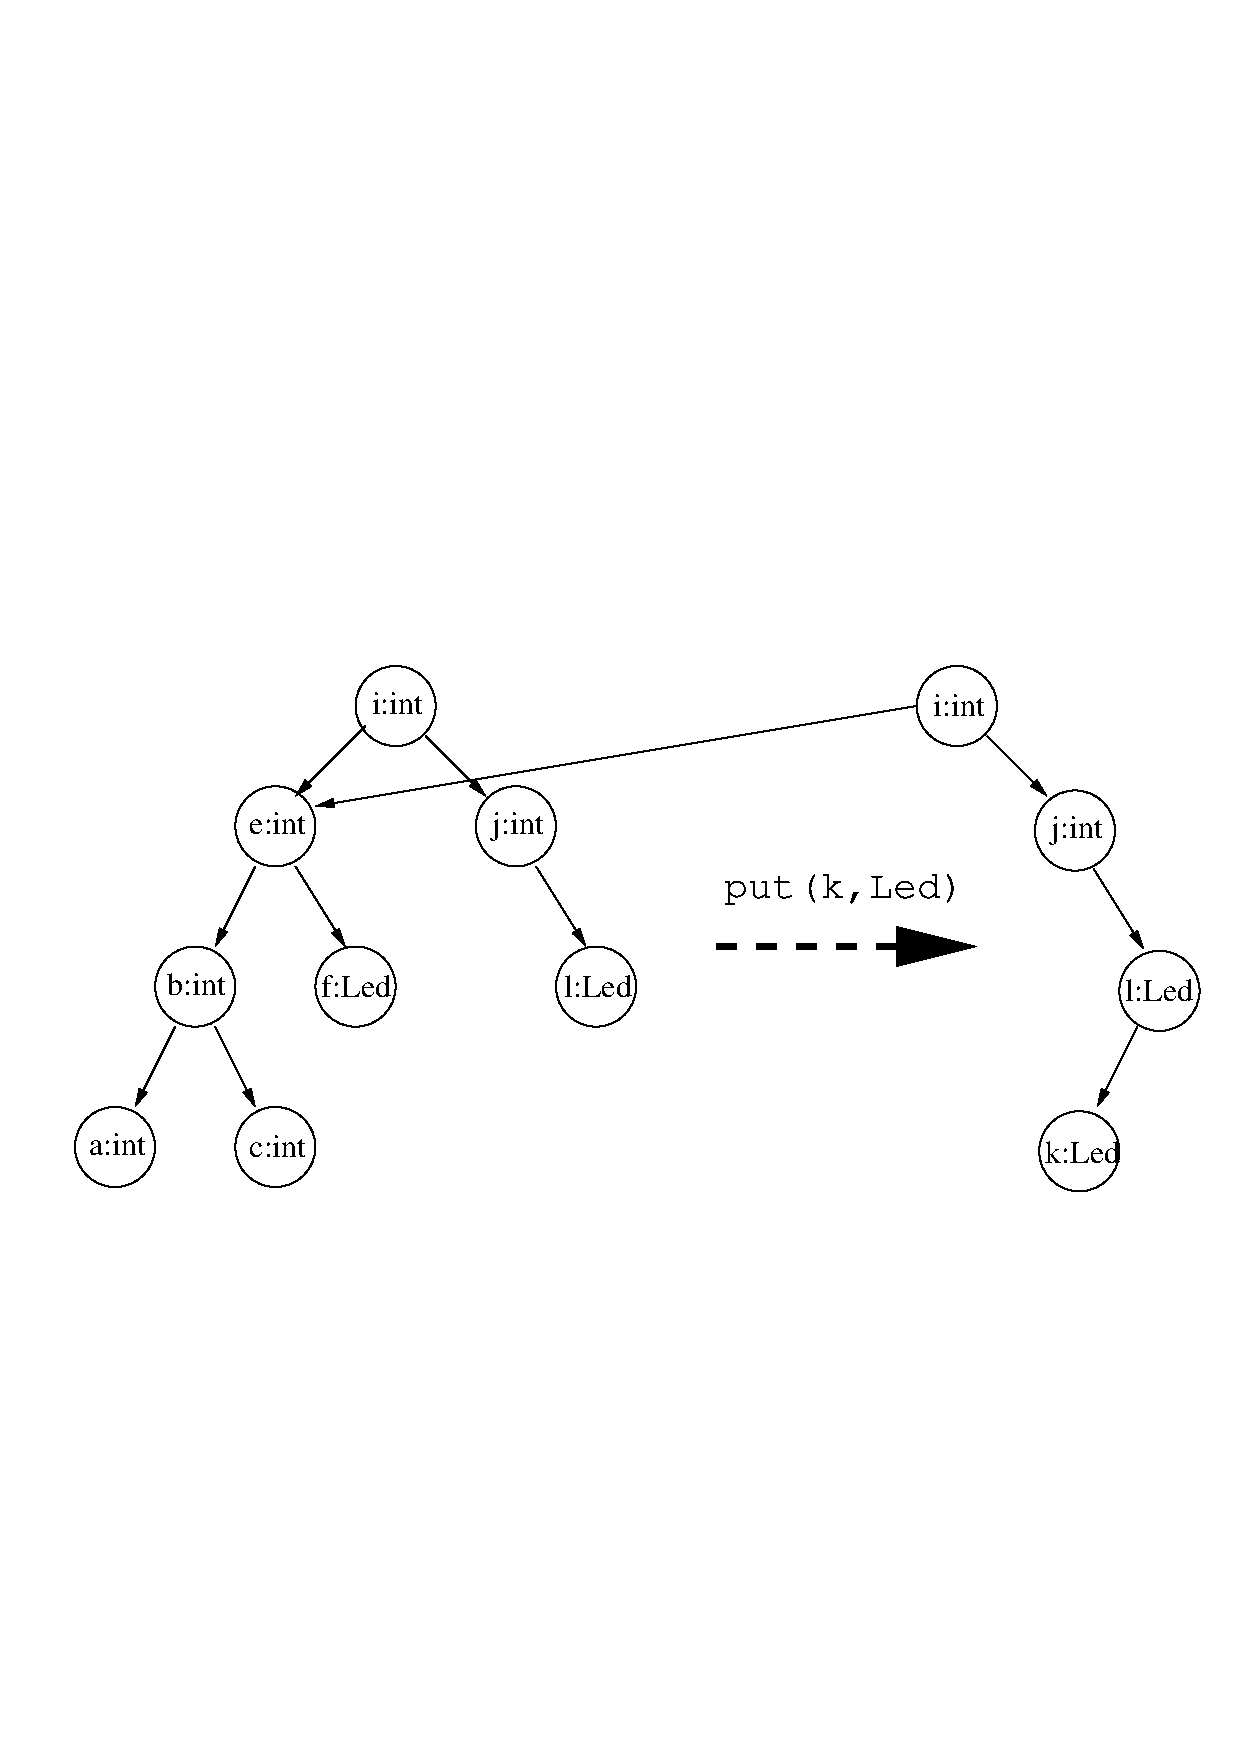
\epsfig{file = insertion.pdf, width = 15cm}
\end{center}
\vspace*{-33ex}
\caption{L'inserzione non distruttiva in un ambiente di un legame per una variabile.}\label{fig:non_destructive}
\end{figure}

\begin{figure}[t]
{\small
\begin{verbatim}
       public class TypeChecker {
         private Table env;
         private ErrorMsg errorMsg;

         private TypeChecker(Table env, ErrorMsg errorMsg) {
           this.env = env; this.errorMsg = errorMsg;
         }
         public TypeChecker(ErrorMsg errorMsg) {
           this(Table.EMPTY,errorMsg);
         }
         public TypeChecker putVar(Symbol var, Type type) {
           return new TypeChecker(env.put(var,type),errorMsg));
         }
         public Type getVar(Symbol var) { return (Type)env.get(var); }
         public void error(int pos, String msg) { errorMsg.error(pos,msg); }
       }
\end{verbatim}
}
\caption{Il type-checker usato per effettuare l'analisi semantica delle espressioni Kitten.}
  \label{fig:semantical.TypeChecker1}
\end{figure}
%
Gli ambienti sono contenuti dentro un \emph{type-checker}, il quale
\e implementato dalla classe \texttt{semantical/TypeChecker.java}
in Figura~\ref{fig:semantical.TypeChecker1}.
Per adesso l'ambiente \`e tutto quello di cui abbiamo bisogno per
effettuare l'analisi semantica delle espressioni,
ma per i comandi aggiungeremo al type-checker ulteriori informazioni
(Sezione~\ref{sec:analysis_commands}).

Possiamo a questo punto implementare le regole
delle Figure~\ref{fig:analysis_expressions1} e~\ref{fig:analysis_expressions2}
tramite una discesa ricorsiva sulla sintassi astratta delle espressioni. In
\texttt{absyn/Expression.java} aggiungiamo:
%
\begin{verbatim}
  private Type staticType;
  private TypeChecker checker;

  public final Type typeCheck(TypeChecker checker) {
    return staticType = typeCheck$0(this.checker = checker);
  }

  protected abstract Type typeCheck$0(TypeChecker checker);
\end{verbatim}
%
Il metodo \texttt{public} e \texttt{final}, di nome \texttt{typeCheck()},
effettua le operazioni comuni a tutte le espressioni, \cioe
l'annotazione del tipo statico inferito per l'espressione e del type-checker
usato per inferirlo. Un metodo ausiliario e \texttt{protected}, di nome
\texttt{typeCheck\$0()}, implementa le operazioni specifiche alla singola
espressione, come specificate nelle Figure~\ref{fig:analysis_expressions1}
e~\ref{fig:analysis_expressions2}.

Vediamo alcuni esempi di implementazione del metodo \texttt{typeCheck\$0()}.
Dentro la classe \texttt{absyn/Variable.java} definiamo:
%
\begin{verbatim}
  protected Type typeCheck$0(TypeChecker checker) {
    Type result = checker.getVar(name);
    if (result == null) return error("undefined variable " + name);
    else return result;
  }
\end{verbatim}
% $
Questa implementazione riflette la specifica in
Figura~\ref{fig:analysis_expressions1}: si cerca la variabile
nell'ambiente; se non esiste si d\`a un errore
altrimenti se ne restituisce il tipo.
Il metodo \texttt{error()} \e definito dentro
\texttt{absyn/Expression.java} come
%
\begin{verbatim}
  protected Type error(String msg) {
    error(checker,msg);
    return Type.INT;
  }
\end{verbatim}
%
Esso stampa il messaggio di errore tramite il type-checker
in utilizzo per l'espressione e ritorna il tipo di emergenza \texttt{int}.
Questo permette di continuare il type-checking anche in presenza di un
errore, bench\'e possa causare degli errori di tipo a cascata.
Il metodo \texttt{error()} a due argomenti \e poi definito dentro
\texttt{absyn/Absyn.java} come
%
\begin{verbatim}
  protected void error(TypeChecker checker, String msg) {
    checker.error(pos,msg);
  }
\end{verbatim}
%
Esso usa il campo \texttt{pos} della sintassi astratta per indicare in che
punto dare l'errore all'utente. Tale campo era il numero di caratteri
passati dall'inizio del file a un punto significativo della parte di sintassi
astratta in considerazione (Sezione~\ref{sec:abstract_syntax_classes}).

Esaminiamo un altro esempio, quello di \texttt{absyn/FieldAccess.java}:
%
\begin{verbatim}
  protected Type typeCheck$0(TypeChecker checker) {
    Type receiverType = receiver.typeCheck(checker);
    if (!(receiverType instanceof ClassType))
      return error("class type required");
    ClassType receiverClass = (ClassType)receiverType;
    if ((field = receiverClass.fieldLookup(name)) == null)
      return error("unknown field " + name);
    return field.getType();
  }
\end{verbatim}
% $
Consistentemente con la Figura~\ref{fig:analysis_expressions1},
tale metodo effettua ricorsivamente l'analisi semantica di
\texttt{receiver} e quindi impone che esso abbia un tipo classe.
Infine cerca il campo di nome \texttt{name} dentro tale tipo classe
e ne restituisce il tipo.

Un altro esempio \e quello di \texttt{absyn/ArrayAccess.java}:
%
\begin{verbatim}
  protected Type typeCheck$0(TypeChecker checker) {
    Type arrayType = array.typeCheck(checker);
    index.mustBeInt(checker);
    if (!(arrayType instanceof ArrayType))
      return error("array type required");
    return ((ArrayType)arrayType).getElementsType();
  }
\end{verbatim}
% $
Consistentemente con la Figura~\ref{fig:analysis_expressions1},
tale metodo effettua ricorsivamente l'analisi semantica di
\texttt{array} e \texttt{index}. Per \texttt{index} usa il metodo ausiliario
\texttt{mustBeInt()} che \e definito dentro \texttt{absyn/Expression.java}
come:
%
\begin{verbatim}
  protected void mustBeInt(TypeChecker checker) {
    if (typeCheck(checker) != Type.INT) error("integer expected");
  }
\end{verbatim}

Consideriamo infine la definizione di \texttt{typeCheck\$0()}
in \texttt{absyn/ArithmeticBinOp.java}:
%
\begin{verbatim}
  protected Type typeCheck$0(TypeChecker checker) {
    Type leftType = getLeft().typeCheck(checker);
    Type rightType = getRight().typeCheck(checker);
    if (leftType.canBeAssignedTo(Type.FLOAT) &&
        rightType.canBeAssignedTo(Type.FLOAT))
      return leftType.leastCommonSupertype(rightType);
    else return error("numerical argument required");
  }
\end{verbatim}
% $
Consistentemente con la Figura~\ref{fig:analysis_expressions2},
esso effettua ricorsivamente l'analisi semantica di
\texttt{left} e \texttt{right} e impone che abbiano un tipo statico
che sia \texttt{float} o un sottotipo di \texttt{float}. Il tipo statico
dell'operazione binaria \e il minimo supertipo comune fra i tipi
statici di \texttt{left} e \texttt{right}.
%
\begin{figure}[t]
\begin{center}
{\small
  \[
    \frac{}
         {\rho\vdash\mathtt{Skip()}:\rho}\qquad
    \frac{\rho\vdash\mathit{condition}:\mathtt{Type.BOOLEAN}\quad
          \rho\vdash\mathit{then}:\rho'\quad
          \rho\vdash\mathit{else}:\rho''}
         {\rho\vdash\mathtt{IfThenElse(\mathit{condition},\mathit{then},
          \mathit{else}):\rho}}
  \]
  \[
    \frac{\mathit{expression}\not=\mathtt{null}\quad
          \rho\vdash\mathit{expression}:t\quad
          \text{il comando occorre in un metodo che ritorna $r$}
          \quad t\le r}
         {\rho\vdash\mathtt{Return(\mathit{expression})}:\rho}
  \]
  \[
    \frac{\text{il comando occorre in un costruttore o in un metodo che
                ritorna \texttt{void}}}
         {\rho\vdash\mathtt{Return(null)}:\rho}
  \]
  \[
    \frac{\rho\vdash\mathit{lvalue}:t_l\quad\rho\vdash\mathit{rvalue}:t_r
          \quad t_r\le t_l}
         {\rho\vdash\mathtt{Assignment(\mathit{lvalue},\mathit{rvalue})}:\rho}
  \]
  \[
    \frac{\rho\vdash\mathit{initialisation}:\rho'\quad
          \rho'\vdash\mathit{condition}:\mathtt{Type.BOOLEAN}\quad
          \rho'\vdash\mathit{update}:\rho''\quad
          \rho'\vdash\mathit{body}:\rho'''}
         {\rho\vdash\mathtt{For(\mathit{initialisation},\mathit{condition},
          \mathit{update},\mathit{body})}:\rho}
  \]
  \[
    \frac{\rho\vdash\mathit{condition}:\mathtt{Type.BOOLEAN}\quad
          \rho\vdash\mathit{body}:\rho'}
         {\rho\vdash\mathtt{While(\mathit{condition},\mathit{body})}:\rho}
  \]
  \[
    \frac{t=\st{\mathit{type}}\quad\rho\vdash\mathit{initialiser}:i\quad 
          i\le t}
         {\rho\vdash\mathtt{LocalDeclaration(\mathit{type},\mathit{name},
          \mathit{initialiser})}:\rho[\mathit{name}\mapsto t]}
  \]
  \[
    \frac{\rho\vdash\mathit{body}:\rho'}
         {\rho\vdash\mathtt{LocalScope(\mathit{body})}:\rho}
    \qquad
     \frac{\begin{array}{c}
       \rho\vdash\mathit{receiver}:\kappa\quad\kappa\in\mathtt{ClassType}
         \quad\rho\vdash\mathit{actuals}:\vec{\tau}\\
       \kappa\mathtt{.methodsLookup(\mathit{name},}\vec{\tau})=
           \{\mathit{method}\}
       \end{array}}
          {\rho\vdash\mathtt{MethodCallCommand(\mathit{receiver},
           \mathit{name},\mathit{actuals})}:\rho}
  \]
  \[
    \frac{\rho\vdash c_1:\rho'\quad\rho'\vdash c_2:\rho''}
         {\rho\vdash c_1;c_2:\rho''}
  \]
}
\end{center}
\caption{Le regole per l'analisi semantica dei comandi Kitten.}
  \label{fig:analysis_commands}
\end{figure}
%
\section{L'analisi semantica dei comandi Kitten}
  \label{sec:analysis_commands}
%
La Figura~\ref{fig:analysis_commands} mostra le regole di analisi semantica
per i comandi Kitten. Questa volta usiamo un giudizio
$\rho\vdash c:\rho'$ il cui significato \e che il comando $c$
eseguito a partire da un ambiente $\rho$ porta in un ambiente $\rho'$.
Questo perch\'e i comandi non hanno un valore ma possono modificare l'ambiente
e le uniche modifiche visibili al livello dei tipi sono quelle dell'insieme
e del tipo delle variabili in scope. In particolare, \e la dichiarazione di una
variabile (la \texttt{LocalDeclaration} in Figura~\ref{fig:analysis_commands})
che estende l'ambiente con una nuova variabile locale, che sostituisce
eventualmente una variabile gi\`a in scope e con lo stesso nome.

Esaminiamo adesso alcune regole della Figura~\ref{fig:analysis_commands}:
%
\begin{description}
\item[\underline{$\mathtt{IfThenElse(\mathit{condition},\mathit{then},\mathit{else})}$}.]
  Il condizionale richiede che la condizione sia un'espressione di tipo
  booleano ed effettua ricorsivamente
  l'analisi semantica di $\mathit{then}$ ed $\mathit{else}$.
  La scelta di lasciare $\rho$ immutato come risultato
  dell'analisi semantica del condizionale implica che eventuali variabili
  locali dichiarate all'interno del ramo \textit{then} o del
  ramo \textit{else} non sono \piu in scope alla fine del condizionale.
\item[\underline{$\mathtt{Return(\mathit{expression})}$}.]
  Il comando di ritorno da metodo o costruttore richiede di effettuare
  ricorsivamente l'analisi semantica dell'espressione ritornata, se esiste.
  Nel caso in cui essa non sia \texttt{null}, allora questo comando deve
  occorrere dentro un metodo che ritorna il tipo statico
  di $\mathit{expression}$ o un suo supertipo. Altrimenti questo comando
  deve occorrere dentro un metodo che ritorna \texttt{void} o dentro
  un costruttore.
\item[\underline{$\mathtt{Assignment(\mathit{lvalue},\mathit{rvalue})}$}.]
  L'analisi semantica dell'assegnamento del valore di un'espressione
  a un leftvalue consiste nel controllare che il tipo statico dell'espressione
  sia lo stesso o un sottotipo del tipo statico del leftvalue.
\item[\underline{$\mathtt{For(\mathit{initialisation},\mathit{condition},
  \mathit{update},\mathit{body})}$}.]
  L'analisi semantica del ciclo \texttt{for} comincia analizzando
  ricorsivamente il comando \textit{initialisation}. Il risultato di questa
  analisi \`e un ambiente $\rho'$, eventualmente arricchito, rispetto a
  $\rho$, con una dichiarazione di una variabile locale al ciclo.
  Si impone poi che \textit{condition} abbia tipo booleano. L'ambiente $\rho'$
  viene usato per effettuare l'analisi
  semantica di \textit{initialisation}, \textit{update} e \textit{body},
  al fine di permettere al programmatore di dichiarare una variabile locale
  dentro \textit{initialisation} e di usarla nelle altre componenti del
  \texttt{for}, come in
  \begin{verbatim}
    for (int i := 0; i < 5; i := i + 1) "".concat(i).output()
  \end{verbatim}
  \vspace*{-2.5ex}
  Se si fosse usato $\rho$ per l'analisi di \emph{condition}, \emph{update} e
  \emph{body},
  la variabile \texttt{i} sarebbe risultata indefinita o avrebbe fatto
  riferimento a un'altra variabile, definita esternamente al ciclo.
\item[\underline{$\mathtt{LocalDeclaration(\mathit{type},\mathit{name},\mathit{initialiser})}$}.]
  L'analisi semantica della dichiarazione di una variabile locale estende
  l'ambiente legando la variabile \textit{name} al tipo semantico di
  \textit{type}. Si effettua anche ricorsivamente
  l'analisi semantica di \textit{initialiser} e si impone che il suo tipo
  statico sia lo stesso o un sottotipo del tipo semantico di \textit{type}.
\item[\underline{$\mathtt{LocalScope(\mathit{body})}$}.]
  L'analisi semantica della creazione di uno scope locale effettua
  ricorsivamente l'analisi semantica del corpo dello scope. Definendo
  $\rho$ come risultato di questa analisi semantica, facciamo in modo che
  eventuali variabili locali dichiarate all'interno del corpo
  non siano \piu visibili all'esterno dello scope. Per esempio, nel comando
  \verb!{ int a; a := 5 }! la variabile
  \texttt{a} non \e \piu visibile dopo la parentesi graffa di chiusura.
\item[\underline{$\mathtt{MethodCallCommand(\mathit{receiver},\mathit{name},\mathit{actuals})}$}.]
  L'analisi semantica del comando di invocazione di metodo \e
  estremamente simile a quella dell'espressioni di invocazione di metodo
  in Figura~\ref{fig:analysis_expressions2}. L'unica differenza \e che qui
  non imponiamo alcun vincolo sul tipo di ritorno del metodo, che pu\`o
  quindi anche essere \texttt{void}.
\item[\underline{$c_1;c_2$}.]
  L'analisi semantica della sequenza di comandi si richiama ricorsivamente
  sui due comandi, usando l'ambiente risultante dall'analisi semantica del
  primo per effettuare l'analisi semantica del secondo. In questo modo
  eventuali variabili locali dichiarate in $c_1$ possono essere usate da $c_2$.
\end{description}
%
\subsection{L'implementazione dell'analisi semantica dei comandi}
  \label{subsec:analysis_commands_implementation}
%
Dal momento
che l'analisi semantica di un comando restituisce un ambiente, implementiamo
il metodo di analisi semantica dentro \texttt{absyn/Command.java} come
%
\begin{verbatim}
  private TypeChecker checker;

  public final TypeChecker typeCheck(TypeChecker checker) {
    checker = typeCheck$0(this.checker = checker);
    if (next != null) return next.typeCheck(checker);
    else return checker;
  }

  protected abstract TypeChecker typeCheck$0(TypeChecker checker);
\end{verbatim}
%
Il metodo \texttt{public} e \texttt{final} di nome \texttt{typeCheck()}
effettua la parte di analisi semantica comune a tutti i comandi, che consiste
nel chiamare il metodo ausiliario \texttt{typeCheck\$0()}, annotare il
type-checker risultante dall'analisi e richiamarsi ricorsivamente sul
comando seguente, se esiste. In questo modo si implementa l'analisi
semantica della sequenza di comandi.

Il metodo \texttt{typeCheck\$0()} effettua la parte di analisi semantica
specifica a ciascun comando, secondo le regole della
Figura~\ref{fig:analysis_commands}. Per esempio, dentro
\texttt{absyn/IfThenElse.java} lo definiamo come
%
\begin{verbatim}
  protected TypeChecker typeCheck$0(TypeChecker checker) {
    condition.mustBeBoolean(checker);
    then.typeCheck(checker);
    else.typeCheck(checker);
    return checker;
  }
\end{verbatim}
% $
Invece dentro \texttt{absyn/For.java} lo definiamo come
%
\begin{verbatim}
  protected TypeChecker typeCheck$0(TypeChecker checker) {
    TypeChecker initChecker = initialisation.typeCheck(checker);
    condition.mustBeBoolean(initChecker);
    update.typeCheck(initChecker);
    body.typeCheck(initChecker);
    return checker;
  }
\end{verbatim}
% $
\begin{figure}[t]
{\small
\begin{verbatim}
public class TypeChecker {
  private Type returnType;    private Table env;   
  private int varNum;         private ErrorMsg errorMsg;

  private TypeChecker(Type returnType, Table env, int varNum, ErrorMsg errorMsg) {
    this.returnType = returnType; this.env = env;
    this.varNum = varNum; this.errorMsg = errorMsg;
  }
  public TypeChecker(Type returnType, ErrorMsg errorMsg) {
    this(returnType,Table.EMPTY,0,errorMsg);
  }
  public TypeChecker setReturnType(Type returnType) {
    return new TypeChecker(returnType,env,varNum,errorMsg);
  }
  public Type getReturnType() { return returnType; }
  public TypeChecker putVar(Symbol var, Type type) {
    return new TypeChecker
      (returnType,env.put(var,new TypeAndNumber(type,varNum)),varNum + 1,errorMsg);
  }
  public Type getVar(Symbol var) {
    TypeAndNumber tan = (TypeAndNumber)env.get(var);
    if (tan != null) return tan.getType(); else return null;
  }
  public int getVarNum(Symbol var) {
    TypeAndNumber tan = (TypeAndNumber)env.get(var);
    if (tan != null) return tan.getNumber(); else return -1;
  }
}
\end{verbatim}
}
\caption{La classe \texttt{semantical/TypeChecker.java} che implementa un type-checker.}
  \label{fig:semantical.TypeChecker}
\end{figure}
%
Si noti in quest'ultimo esempio come l'ambiente (in effetti, il type-checker)
risultante dall'analisi di \texttt{initialisation} sia poi usato per effettuare
l'analisi semantica di \texttt{condition}, \texttt{update} e \texttt{body},
conformemente alla Figura~\ref{fig:analysis_commands}.

La Figura~\ref{fig:semantical.TypeChecker} mostra una revisione del
type-checker della Figura~\ref{fig:semantical.TypeChecker1}.
Adesso esso conosce il tipo di ritorno del metodo che
si sta analizzando, fornito al momento della
costruzione del type-checker tramite l'unico costruttore pubblico
in Figura~\ref{fig:semantical.TypeChecker} e usato poi per
implementare l'analisi semantica dei comandi \texttt{return}: in
\texttt{absyn/Return.java} definiamo infatti:
%
\begin{verbatim}
  protected TypeChecker typeCheck$0(TypeChecker checker) {
    Type expectedReturnType = checker.getReturnType();
    if (returned == null && expectedReturnType != Type.VOID)
      error("missing return value");
    if (returned != null &&
        !returned.typeCheck(checker).canBeAssignedTo(expectedReturnType))
      error("illegal return type: " + expectedReturnType + " expected");
    return checker;
  }
\end{verbatim}
% $
conformemente alla Figura~\ref{fig:analysis_commands}.

Si noti che il type-checker in Figura~\ref{fig:semantical.TypeChecker} associa
alle variabile dell'ambiente non solo il loro tipo di dichiarazione,
ma anche un numero progressivo, che sar\`a utile in fase di generazione del
codice (Capitolo~\ref{chap:translate}).
%
\section{L'analisi semantica delle classi Kitten}
  \label{sec:analysis_classes}
%
Fare l'analisi semantica di una classe Kitten significa effettuare
l'analisi semantica dei suoi membri, \cioe campi, costruttori e metodi.
Nulla va controllato per quanto riguarda i campi. Per quanto riguarda
costruttori e metodi, invece, occorre effettuare l'analisi semantica
del loro corpo. Essendo il loro corpo un comando, possiamo usare a tal
fine le regole della Figura~\ref{fig:analysis_commands}, cominciando
l'analisi da un ambiente iniziale in cui i parametri del costruttore o del
metodo sono legati al loro tipo di dichiarazione (incluso il parametro
implicito \texttt{this}). A tal fine, definiamo una funzione che
aggiunge a un ambiente una lista di variabili dichiarate come parametri
formali:
%
\begin{align*}
  \rho+{\mathtt{null}}&=\rho \\
  \rho+{\mathtt{FormalParameters(\mathit{type},\mathit{name},\mathit{next})}}&=(\rho+{\mathit{next}})[\mathit{name}\mapsto\st{type}]
\end{align*}
%
L'analisi semantica di un costruttore o metodo con parametri formali
$\mathit{formals}$ e dichiarato in una classe
il cui tipo semantico \`e $\kappa$ viene quindi effettuata
a partire da un ambiente iniziale
\[
  \overline{\rho}=[\mathtt{this}\mapsto\kappa]+{\mathit{formals}}
\]
Se $\mathit{body}$ \`e il corpo del costruttore o metodo, si tratter\`a
di verificare che il giudizio $\overline{\rho}:\mathit{body}:\rho'$ sia
valido per un qualche $\rho'$.

Anche il metodo che fa l'analisi semantica dei membri di una classe si
chiama \texttt{typeCheck()}. Esso \`e definito dentro
\texttt{absyn/ClassMemberDeclaration.java} come
%
\begin{verbatim}
  final void typeCheck(ClassType currentClass) {
    typeCheck$0(currentClass);
    if (next != null) next.typeCheck(currentClass);
  }

  protected abstract void typeCheck$0(ClassType currentClass);
\end{verbatim}
% $
ovvero tramite il solito metodo \texttt{final} che richiama, su tutta la
lista dei membri della classe, il metodo ausiliario
\texttt{typeCheck\$0()} che effettua l'analisi specifica a ciascun membro.
Abbiamo detto che l'analisi semantica dei campi non richiede nessun controllo:
dentro la classe di sintassi astratta
\texttt{absyn/FieldDeclaration.java} definiamo quindi:
%
\begin{verbatim}
  protected void typeCheck$0(ClassType currentClass) {}
\end{verbatim}
% $
In \texttt{absyn/ConstructorDeclaration.java} definiamo invece:
%
\begin{verbatim}
  protected void typeCheck$0(ClassType currentClass) {
    TypeChecker checker
      = new TypeChecker(Type.VOID,currentClass.getErrorMsg());
    checker = checker.putVar(Symbol.THIS,currentClass);
    if (getFormals() != null) checker = getFormals().typeCheck(checker);
    getBody().typeCheck(checker);
    getBody().checkForDeadcode();
  }
\end{verbatim}
% $
Questo metodo comincia col costruire un type-checker con ambiente vuoto e
che si aspetta come tipo di ritorno \texttt{Type.VOID}. Quindi aggiunge
la variabile \texttt{this} legata al tipo semantico
della classe e i parametri formali legati al loro tipo di dichiarazione,
rispecchiando la definizione precedente di $\overline{\rho}$.
Infine effettua il type-checking del corpo del costruttore e controlla che al
suo interno non ci sia del codice morto (Sezione~\ref{sec:dead_code}).
Il ragionamento \e simile nel caso della dichiarazione di un metodo,
ma si usa il tipo di ritorno del metodo al posto di \texttt{Type.VOID} e si
controlla che se il metodo ne ridefinisce un
altro di una superclasse allora la ridefinizione del tipo di ritorno
soddisfi il test \texttt{canBeAssignedToSpecial()}
visto in Sezione~\ref{sec:semantical_types}. Se inoltre il metodo non
ritorna \texttt{void}, si impone che il valore di ritorno del metodo
\texttt{checkForDeadcode()} sia \texttt{true}, in modo da garantire che
il metodo termini sempre con un comando \texttt{return}.

\greycomment{
L'analisi semantica di Kitten descritta in questo capitolo \e un po'
semplificata rispetto alla realt\`a. In particolare non abbiamo considerato
come dall'analisi della classe di partenza
(Sezione~\ref{sec:analysis_classes}) si arrivi a quella
delle altre classi a cui essa fa riferimento. Questo \e ottenuto
facendo in modo che le regole delle Figure~\ref{fig:analysis_expressions1},
\ref{fig:analysis_expressions2} e~\ref{fig:analysis_commands}, quando
hanno bisogno di ottenere il tipo semantico delle espressioni di tipo,
richiamino ricorsivamente il type-checking su tutte le classi che vi occorrono.
Al fine di evitare cicli, si usa un flag
\texttt{typeChecked} all'interno di \texttt{types.ClassType}.}
%
\begin{exercise}\label{ex:conditional_expression}
Si aggiunga alle espressioni la sintassi astratta di un'\emph{espressione
condizionale}
$\mathit{exp}_1\mathtt{?}\,\mathit{exp}_2\,\mathtt{:}\,\mathit{exp}_3$
che restituisce il valore di $\mathit{exp}_2$ se $\mathit{exp}_1$ \e
vera e il valore di $\mathit{exp}_3$ altrimenti. Si dia la sua regola di
type-checking.
\end{exercise}
%
\begin{exercise}\label{ex:switch}
Si aggiunga ai comandi la sintassi astratta di un comando \texttt{switch}.
Non ci si limiti a espressioni costanti nei vari casi.
Si dia la regola di type-checking per tale comando.
\end{exercise}
%
\begin{exercise}\label{ex:break_continue}
Si aggiunga ai comandi la sintassi astratta dei comandi
\texttt{break} e \texttt{continue}. Si diano le loro regole di type-checking,
che devono garantire che tali comandi occorrano solo dentro un ciclo.
Come modifichereste il type-checker in Figura~\ref{fig:semantical.TypeChecker}
in modo da implementare tali controlli?
\end{exercise}
